\documentclass[11pt]{article}

\usepackage[a4paper,margin=2.35cm]{geometry}
\usepackage{booktabs}
\usepackage{array}
\usepackage{tabularx}
\usepackage{graphicx}
\usepackage{float}
\usepackage{caption}
\usepackage{xcolor}
\usepackage{enumitem}
\usepackage{amsmath}
\usepackage{amssymb}
\usepackage{hyperref}
\usepackage{microtype}

\definecolor{chapterblue}{HTML}{2F5F85}
\definecolor{textgray}{HTML}{333333}

\graphicspath{{../../charts/}}
\hypersetup{
  colorlinks=true,
  linkcolor=chapterblue,
  urlcolor=chapterblue,
  citecolor=chapterblue
}
\captionsetup{font=small,labelfont=bf}
\setlist[itemize]{leftmargin=1.6em,itemsep=0.15em}
\setlength{\parindent}{0pt}
\setlength{\parskip}{0.65em}
\renewcommand{\arraystretch}{1.18}

\title{\textbf{Part 6: Quantitative Modeling, State Dependence, and Risk Extension}}
\author{DASE7337 Group Project: Airline Delay and Cancellation Operational Risk}
\date{April 2026}

\begin{document}
\maketitle

\setcounter{section}{5}

\section{Frequency, Severity, and Model Selection}

\subsection{Purpose of the Quantitative Layer}
The previous chapter prepared the BTS data for modeling by cleaning the source file, standardizing the variables, and separating airline-month from airport-month views. This chapter turns that dataset into a formal risk framework. The sequence follows the course logic closely. Frequency modeling asks how often disruption occurs. Severity modeling asks how large the average operational impact becomes once disruption occurs. State dependence asks whether stressed operating conditions persist from one month to the next. Annual aggregate simulation then combines those pieces into a yearly loss distribution, while the tail extension and sensitivity analysis test whether the main conclusions still hold once attention moves to extremes and targeted shocks.

The loss proxy is measured in \textit{delay-equivalent minutes} rather than money. The reason is straightforward. The BTS data record delay minutes, cancellations, and diversions directly, but they do not contain a consistent financial loss for each event. Translating minutes into money would therefore require a separate pricing layer and another set of assumptions. To keep the link between observed data and modeled loss transparent, the project stays in minutes and treats the framework as operational risk rather than financial loss.

\subsection{Why Candidate Distributions Are Compared}
The project does not impose one distribution from the start. Instead, it compares a small set of course-consistent candidates for each type of variable. That choice reflects two practical considerations. First, the data combine routine months with genuinely stressed months, so the same variable may plausibly show more than one right-skewed or over-dispersed pattern. Second, the goal is not just to fit a statistic well. It is to choose a distribution that makes sense statistically and still reads sensibly as an operational-risk model.

For frequency variables, the candidates are Poisson and Negative Binomial. For severity variables, the candidates are Lognormal and Weibull. These are not arbitrary choices. Each pair reflects the course distinction between a parsimonious benchmark model and a more flexible alternative. The benchmark is valuable because it gives a clean reference point; the flexible model is valuable because airport operations often exhibit clustering, heterogeneity, and tail amplification.

\subsection{AIC as the Model-Selection Criterion}
The project selects between candidate distributions using the Akaike Information Criterion (AIC). AIC is defined as
\[
\mathrm{AIC}=2k-2\log(\hat{L}),
\]
where \(k\) is the number of estimated parameters and \(\hat{L}\) is the maximized likelihood of the fitted model.

Conceptually, AIC rewards fit but penalizes unnecessary complexity. A lower AIC therefore indicates a better balance between explanatory power and parsimony within the candidate set being compared.

AIC is not a significance test and does not produce a p-value. It is a relative model-comparison tool. That is exactly why it fits this project. The task here is not to prove that one distribution is "statistically significant" in isolation. It is to choose, from a small set of plausible candidates, the specification that represents the data most convincingly.

Relative to the simpler model-comparison logic used in many classroom examples, AIC has three advantages for this project. First, it can compare non-nested models, which is essential when Lognormal and Weibull are both plausible but structurally different. Second, it penalizes unnecessary complexity automatically, which is useful when the more flexible model might otherwise dominate by fit alone. Third, it creates a unified decision rule that can be applied consistently across both frequency and severity blocks. In that sense, AIC operationalizes the course idea of calibration and model verification into one explicit, reproducible step.

The model-selection process therefore follows the same sequence for each variable:
\begin{enumerate}
  \item identify the variable type and select the relevant candidate distributions;
  \item estimate the parameters of each candidate model by maximum likelihood;
  \item compute the AIC for each fitted model;
  \item choose the model with the lower AIC;
  \item interpret the selected model in operational terms rather than stopping at the numeric fit criterion.
\end{enumerate}

\subsection{Frequency Modeling}
The first empirical layer focuses on count-type disruption variables observed at the airline-month level. Six variables are modeled: total delayed arrivals, cancellations, diversions, internal airline-operational disruption counts, system/NAS disruption counts, and external shock disruption counts. These are natural loss-number variables because they count how many disruption events occur within a fixed observation window.

The Poisson model provides the homogeneous benchmark:
\[
\mathbb{P}(N=n)=e^{-\lambda}\frac{\lambda^n}{n!}, \qquad n=0,1,2,\dots
\]
Under this structure, the event intensity is relatively stable, and the mean and variance are close.

The Negative Binomial model provides the flexible alternative:
\[
\mathbb{P}(N=n)=\frac{\Gamma(n+r)}{\Gamma(r)\,n!}p^r(1-p)^n,
\qquad n=0,1,2,\dots
\]
This model allows variance to exceed the mean, which makes it suitable when disruption events cluster into high-pressure months rather than arriving evenly over time.

This distinction matters operationally. If airport disruption behaved like a Poisson process, planning could focus on a relatively stable average load. If it behaves more like a Negative Binomial process, average load is not enough. Resilience planning also has to account for concentration, spikes, and stressed regimes.

\begin{table}[H]
\centering
\caption{Selected frequency models}
\begin{tabular}{lrrrr}
\toprule
Variable & Selected model & AIC & Normal mean & Disrupted mean \\
\midrule
Total delay count & Negative Binomial & 7290.82 & 207.13 & 340.87 \\
Cancellation count & Negative Binomial & 4463.27 & 14.15 & 84.36 \\
Diversion count & Negative Binomial & 2531.80 & 2.60 & 5.30 \\
Internal ops count & Negative Binomial & 6766.28 & 132.65 & 204.68 \\
System ops count & Negative Binomial & 6047.51 & 68.42 & 124.20 \\
External ops count & Negative Binomial & 3502.99 & 6.06 & 12.00 \\
\bottomrule
\end{tabular}
\end{table}

The pattern is consistent across all six count variables: each is better fitted by the Negative Binomial model. That means over-dispersion is not confined to one corner of the disruption system. JFK disruption does not look like a smooth random arrival process. It looks like a system with clustering, pressure accumulation, and uneven monthly burden.

\begin{figure}[H]
\centering
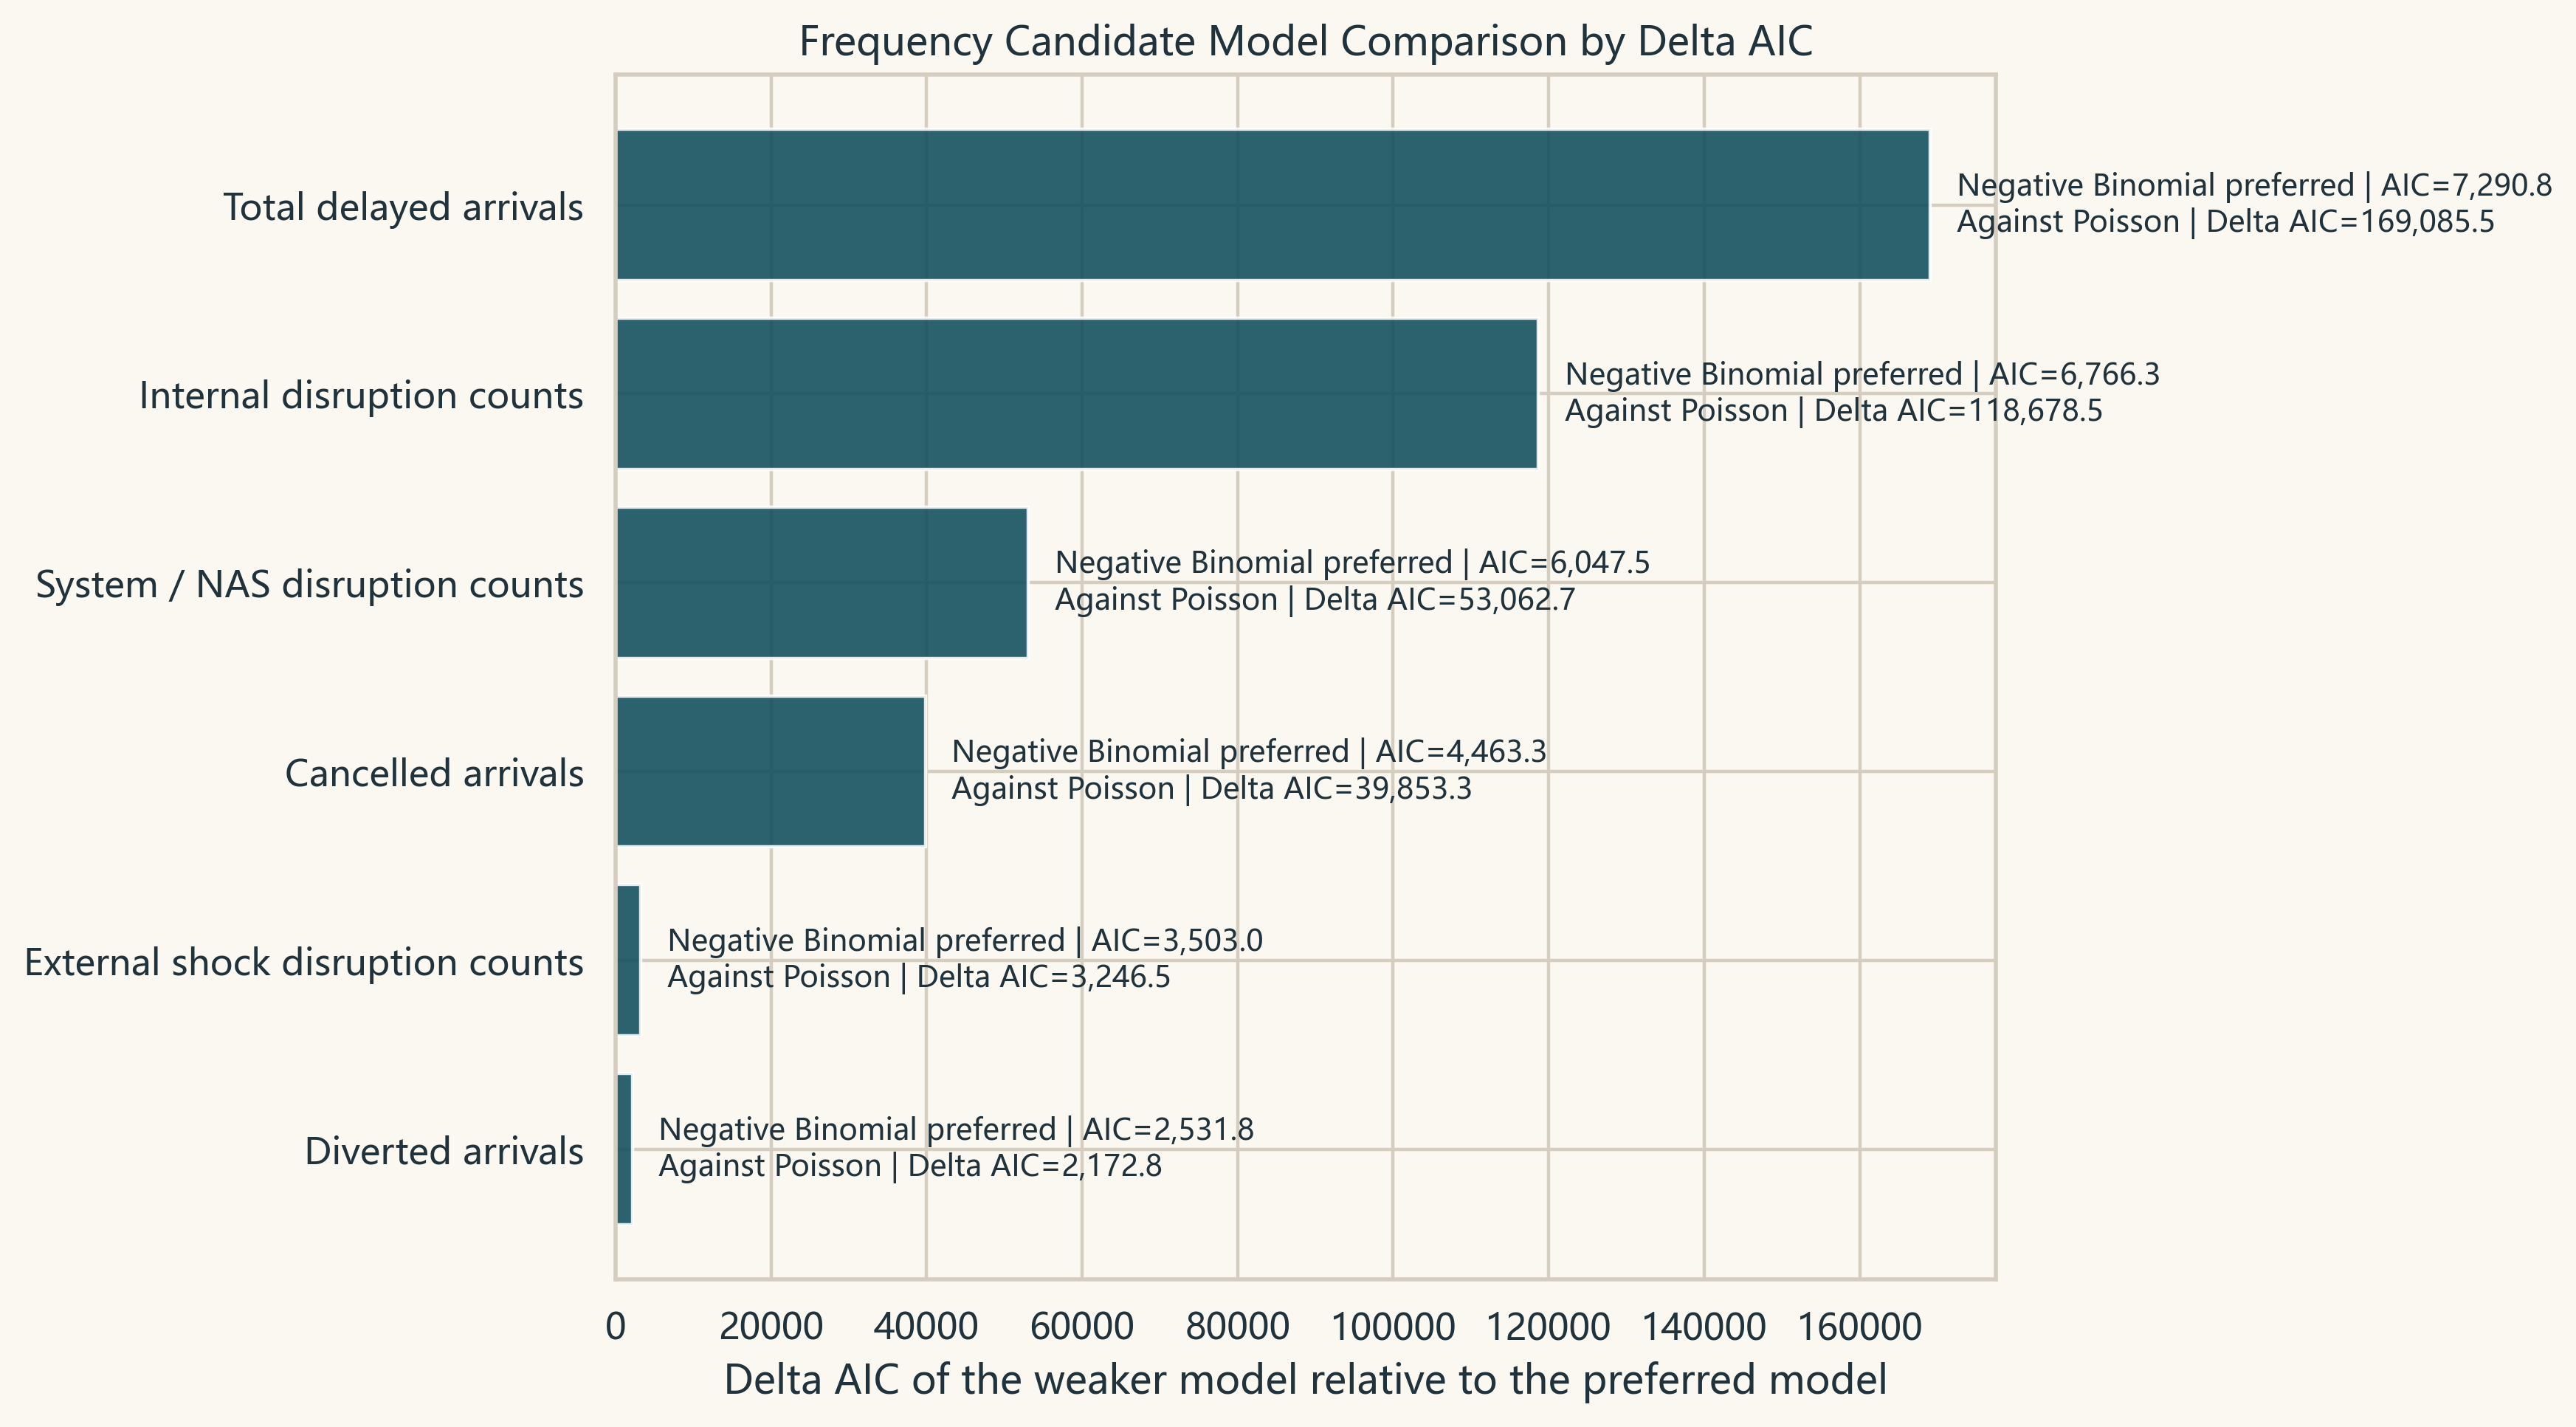
\includegraphics[width=0.92\linewidth]{chart_8_frequency_aic_comparison_en.png}
\caption{AIC comparison for candidate frequency models}
\label{fig:freq-aic-en}
\end{figure}

Figure~\ref{fig:freq-aic-en} shows the same result visually. For every count block, the Negative Binomial AIC is lower than the Poisson AIC. The point is not just that one number beats another. The point is that the same modeling message appears across the whole count layer: operational disruption counts are clustered rather than loosely fluctuating around a stable monthly mean.

\subsection{Severity Modeling}
The second quantitative layer studies how large the operational impact becomes once disruption occurs. Since the project uses a minutes-based loss proxy, severity is defined as average delay minutes per disruption event. Four severity variables are modeled: total average delay minutes, internal average minutes, system average minutes, and external average minutes.

Two candidate distributions are compared. The Lognormal model is appropriate when severity is non-negative, right-skewed, and plausibly generated by multiplicative amplification:
\[
X \sim \mathrm{Lognormal}(\mu,\sigma^2)
\quad \Longleftrightarrow \quad
\log X \sim \mathcal{N}(\mu,\sigma^2).
\]

The Weibull model is also non-negative and right-skewed, but it is often more suitable when the severity pattern appears operationally bounded:
\[
f(x)=\frac{k}{\lambda}\left(\frac{x}{\lambda}\right)^{k-1}
e^{-(x/\lambda)^k}, \qquad x\ge 0.
\]

The reason for comparing these two models is not only statistical but also interpretive. A Lognormal pattern suggests that a sequence of multiplicative frictions can compound average disruption size. A Weibull pattern suggests that severity still has a long right tail, but its shape is more constrained by operational limits such as scheduling buffers, airport capacity, and recovery procedures.

\begin{table}[H]
\centering
\caption{Selected severity models}
\begin{tabular}{lrrrr}
\toprule
Variable & Selected model & AIC & Normal mean & Disrupted mean \\
\midrule
Total avg delay minutes & Weibull & 5146.84 & 67.47 & 76.76 \\
Internal avg minutes & Lognormal & 5362.19 & 78.28 & 83.24 \\
System avg minutes & Lognormal & 4413.72 & 47.83 & 65.53 \\
External avg minutes & Lognormal & 4864.21 & 103.71 & 111.83 \\
\bottomrule
\end{tabular}
\end{table}

The total severity measure is best fitted by a Weibull distribution, whereas the three disruption blocks are best fitted by Lognormal distributions. This pattern is plausible. At the system-wide level, average delay severity appears right-skewed but still shaped by operating constraints. At the block level, internal, system, and external severity seem more consistent with multiplicative escalation, especially in stressed conditions.

The state split is informative as well. Every severity measure is higher in disrupted months than in normal months, and the increase is especially visible for the system/NAS block. In other words, disrupted months are not simply months with more events. They are also months in which each event tends to be more damaging. That is one reason the later aggregate model needs frequency, severity, and state dependence together.

\begin{figure}[H]
\centering
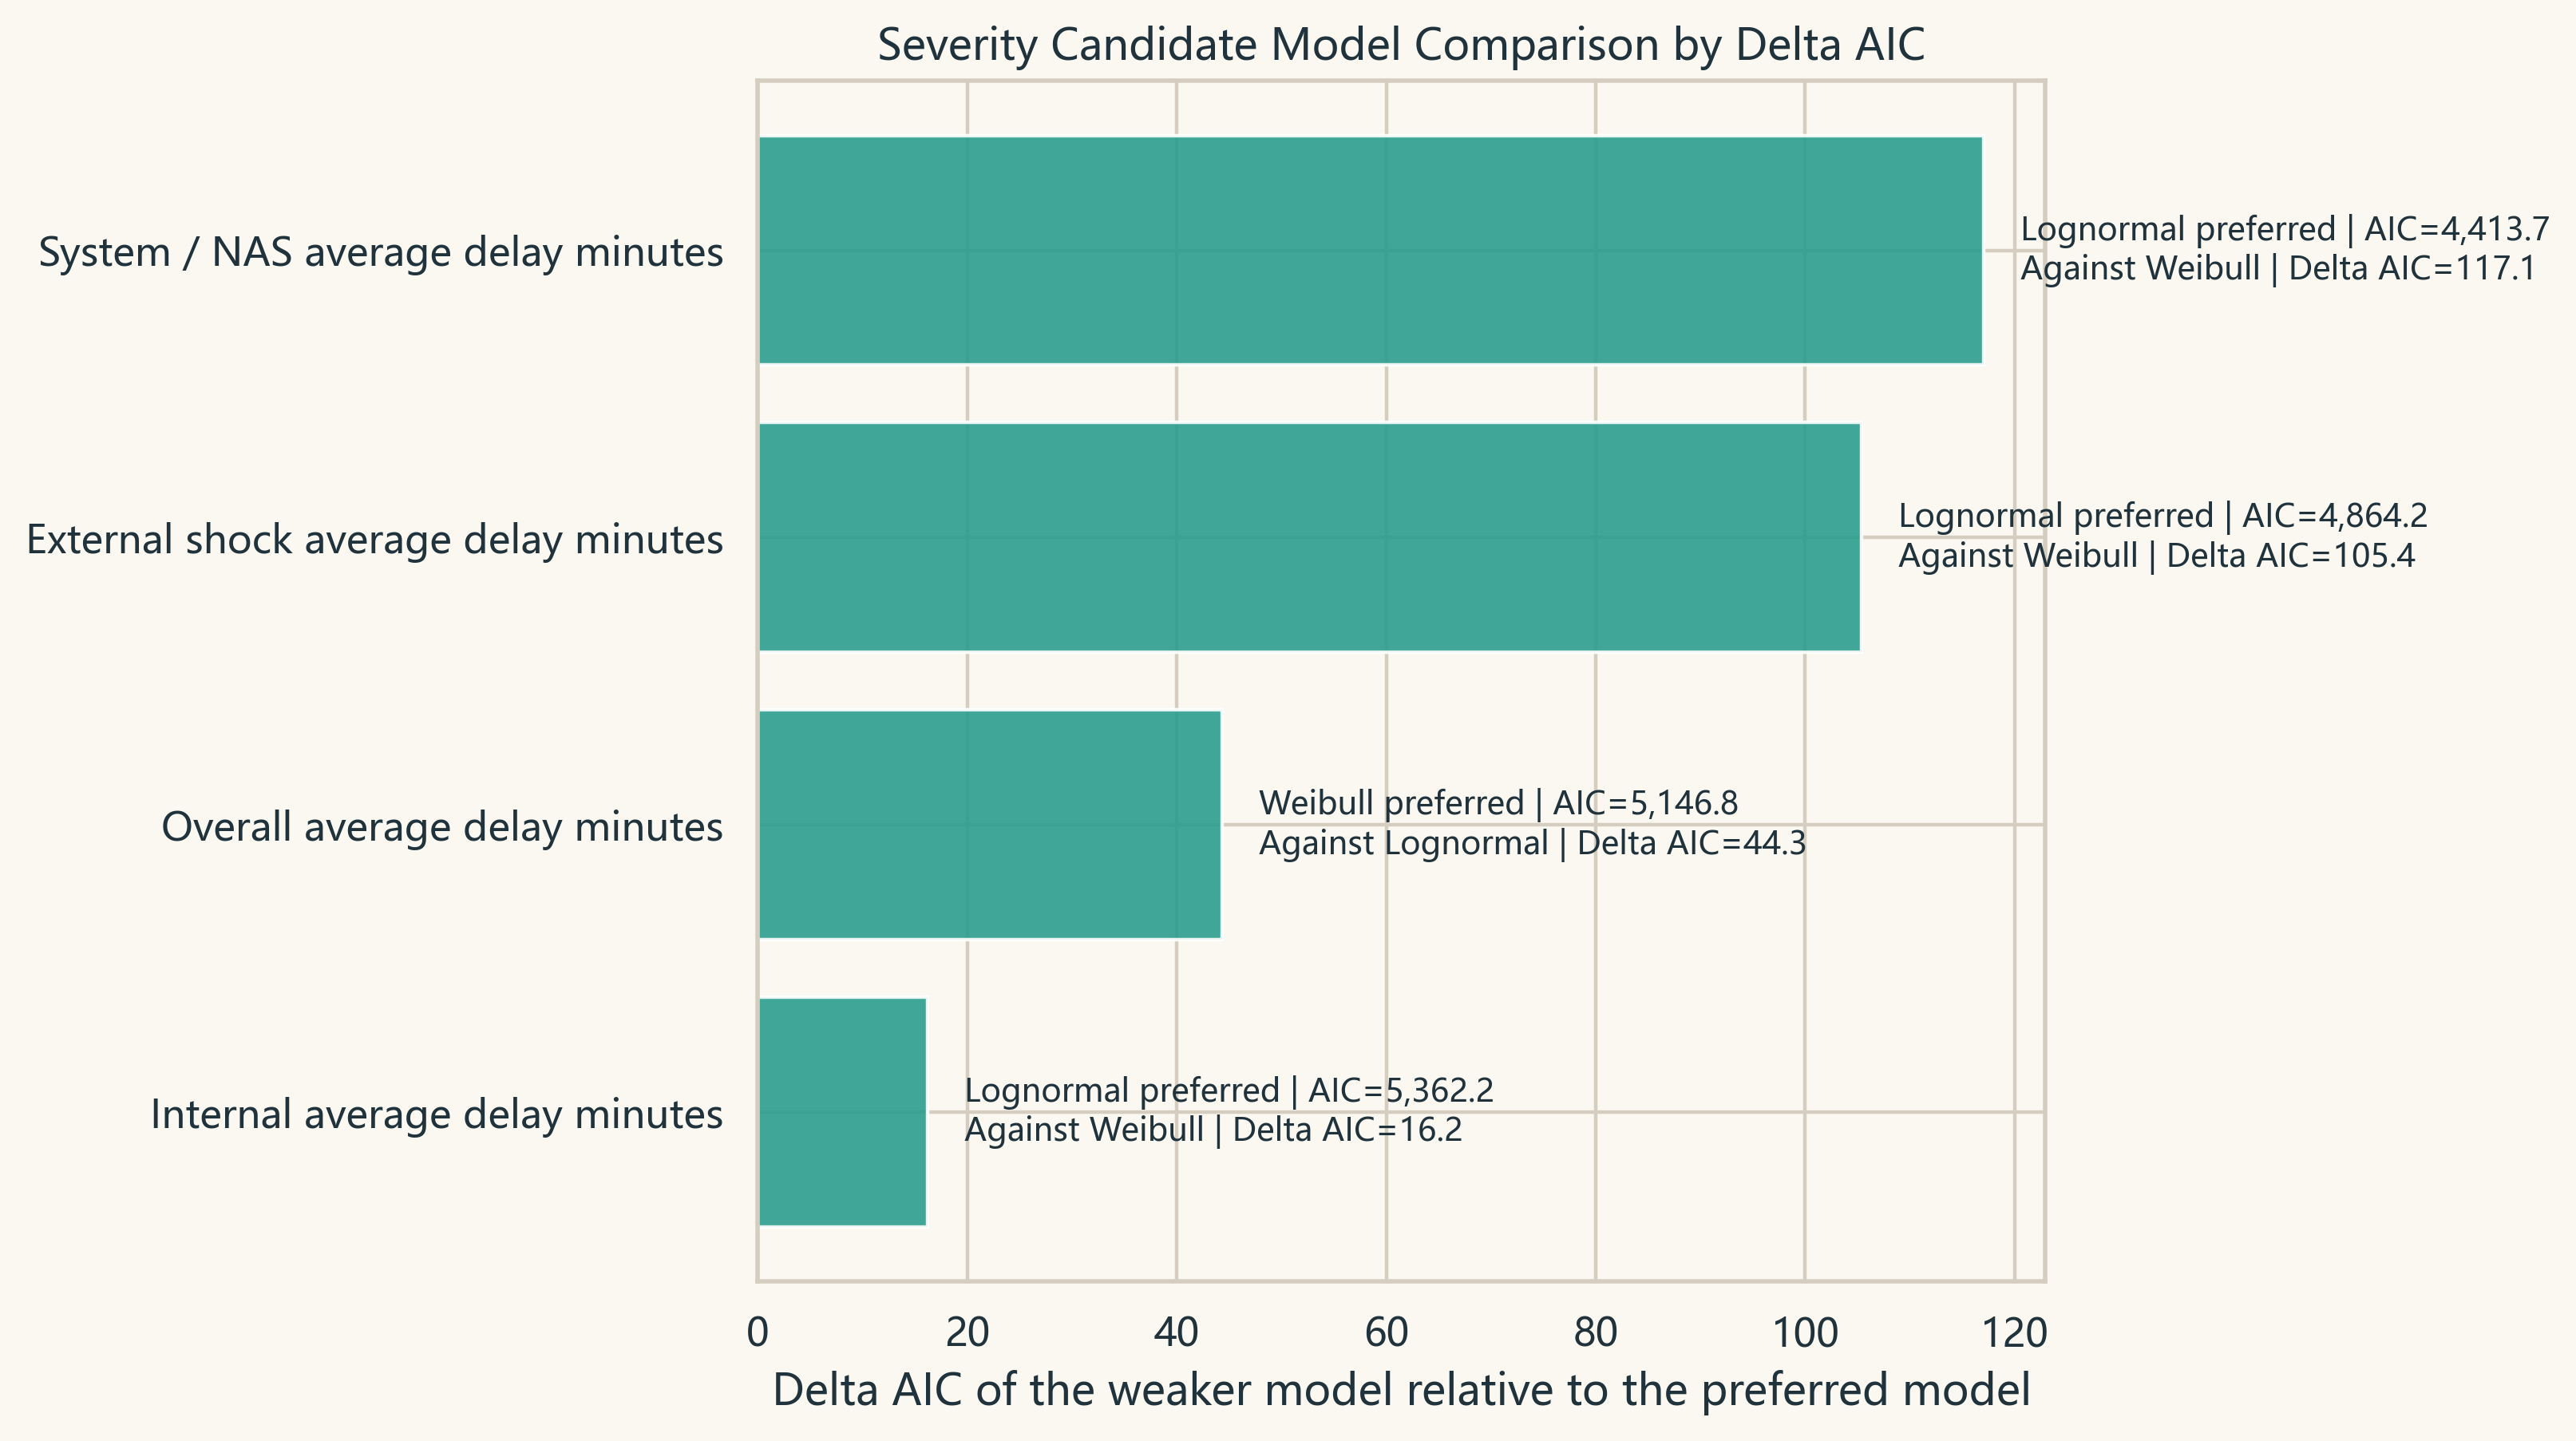
\includegraphics[width=0.92\linewidth]{chart_9_severity_aic_comparison_en.png}
\caption{AIC comparison for candidate severity models}
\label{fig:sev-aic-en}
\end{figure}

\section{State Definition and Markov Dependence}

\subsection{Why State Dependence Is Needed}
Frequency and severity alone describe how often disruptions occur and how large they are once they occur. However, they do not yet explain whether operating conditions are persistent across time. Airport operations are not reset to a neutral baseline every month. A month with high congestion, cancellations, and accumulated delay can make the following month more vulnerable as well. For that reason, the project introduces a state-based layer at the airport-month level.

The two states are defined as \textit{Normal} and \textit{Disrupted}. The modeling idea is intentionally simple: rather than building a large latent-state system, the project asks whether a parsimonious two-state regime is sufficient to capture persistence in operating stress.

\subsection{Competing State Rules}
Two candidate state-definition rules are compared. The first is a simple impact-threshold rule:
\[
\text{Disrupted}_t = \mathbf{1}\{ \text{Impact}_t \ge Q_{0.75}(\text{Impact}) \}.
\]
This rule is transparent, but it uses only one dimension of stress.

The second is a composite rule that combines delay rate, cancellation rate, and total disruption impact:
\[
S_t = z(\text{DelayRate}_t) + z(\text{CancelRate}_t) + z(\text{Impact}_t),
\]
and defines month \(t\) as disrupted when \(S_t\) lies above the empirical 75th percentile threshold.

The reason for comparing these two rules is substantive. If the state is defined only by total impact, then a single dimension dominates the classification. If the state is defined by a composite score, the state captures multiple symptoms of operational stress at once. The final rule must therefore be judged not only by intuition, but also by year-to-year stability.

\begin{table}[H]
\centering
\caption{Comparison of candidate disrupted-state rules}
\begin{tabular}{lrrr}
\toprule
Rule & Disrupted share & Yearly std. dev. & Selected \\
\midrule
Impact 75\% threshold & 0.25 & 0.1863 & No \\
Delay-cancel-impact composite & 0.25 & 0.1521 & Yes \\
\bottomrule
\end{tabular}
\end{table}

The composite rule is selected because it produces a more stable disrupted share across years while preserving the same overall 25\% state frequency. That makes it easier to defend on both substantive and empirical grounds. It reflects multiple symptoms of operating stress, and it behaves more steadily across the sample than the simpler impact-only rule.

\subsection{Why a Markov Chain Is Appropriate}
Once the monthly states are defined, the project models transitions across months using a first-order two-state Markov chain. This choice is justified by the operational setting. If disruption states were independent across months, then knowing whether the current month is normal or disrupted would add little information about the next month. In contrast, if high-stress periods persist, then the current state should help predict the next one.

The Markov framework formalizes this idea through transition probabilities:
\[
P_{ij}=\mathbb{P}(X_{t+1}=j \mid X_t=i),
\qquad i,j\in\{N,D\}.
\]
The empirical transition matrix is estimated from the sequence of airport-month states.

\begin{table}[H]
\centering
\caption{Estimated two-state transition matrix}
\begin{tabular}{llr}
\toprule
Current state & Next state & Probability \\
\midrule
Normal & Normal & 0.8148 \\
Normal & Disrupted & 0.1852 \\
Disrupted & Normal & 0.5294 \\
Disrupted & Disrupted & 0.4706 \\
\bottomrule
\end{tabular}
\end{table}

The key comparison is between \(P(D\to D)\) and \(P(N\to D)\). The probability of remaining in disruption is much higher than the probability of entering disruption from a normal month. This does not establish a full structural theory of airport operations, but it does give meaningful empirical evidence of monthly persistence. For the purposes of this project, that is enough to justify a simple regime-based dependence layer.

\begin{figure}[H]
\centering
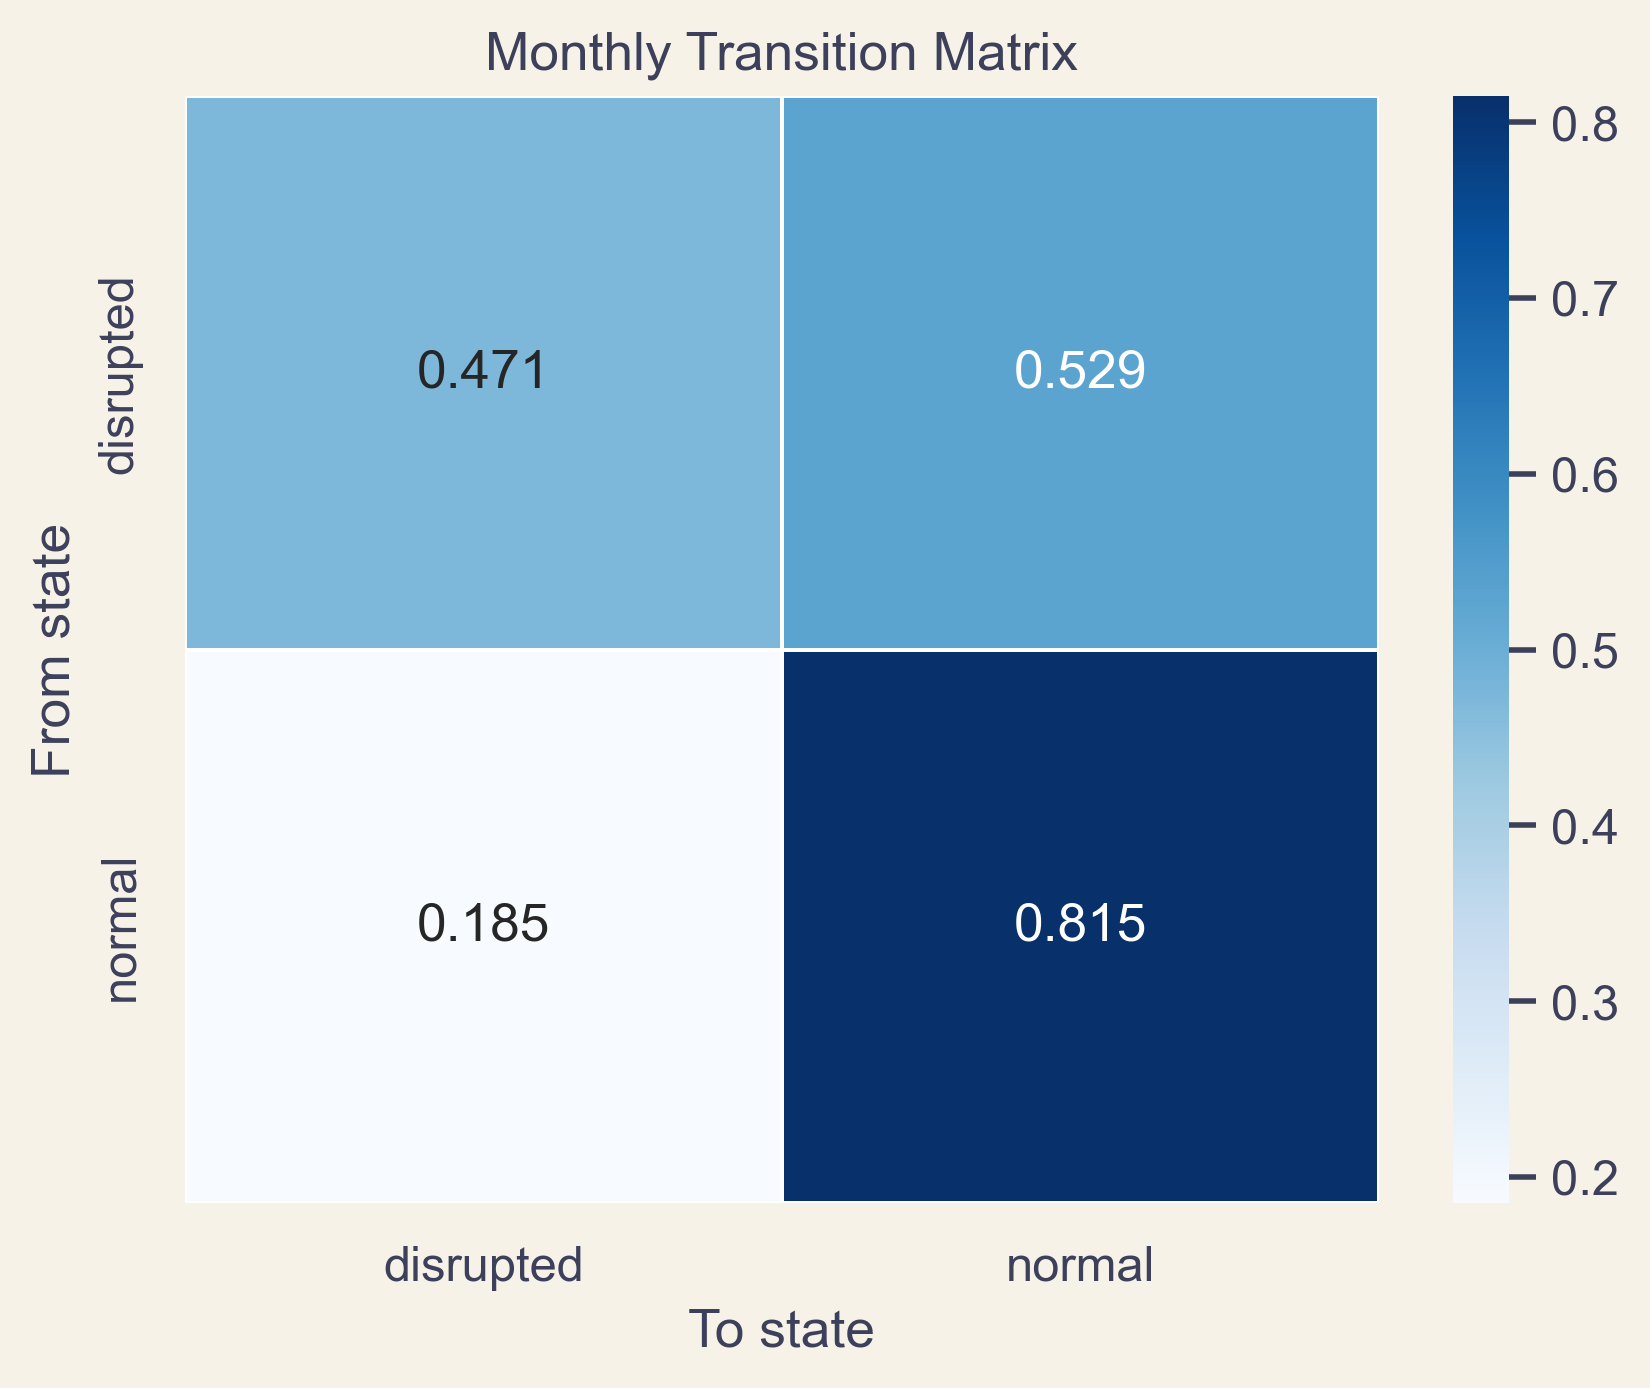
\includegraphics[width=0.52\linewidth]{chart_7_markov_transition_matrix.png}
\caption{Two-state Markov transition matrix}
\label{fig:markov-en}
\end{figure}

The Markov layer therefore adds something that neither the count models nor the severity models can provide on their own. It gives the project a way to distinguish between isolated bad months and stress regimes that tend to continue once they have started.

\section{Annual Aggregate Risk and EVT Tail Extension}

\subsection{From Monthly Components to Annual Risk}
After the frequency, severity, and dependence layers are estimated, the project combines them into annual aggregate operational risk. The monthly impact proxy is defined in delay-equivalent minutes as
\[
L_t = \text{DelayMinutes}_t + 180 \times \text{Cancelled}_t + 240 \times \text{Diverted}_t.
\]
Annual impact is then obtained by summing across the 12 simulated months:
\[
L^{(A)} = \sum_{t=1}^{12} L_t.
\]

This aggregation step is central to the report. Up to this point, each model describes one component of the loss process. The annual simulation integrates them into a single operational-risk distribution that can be summarized by expected impact, VaR, and TVaR. In practical terms, the model does not simulate one ``representative month'' and then scale it by twelve. Instead, it simulates a full path of 12 monthly states, monthly disruption counts, and monthly severity outcomes, and then accumulates them into annual impact. The annual distribution is therefore path-based rather than a simple static extrapolation.

More formally, let \(S_t \in \{N,D\}\) denote the operating state in month \(t\), where \(N\) is Normal and \(D\) is Disrupted. Conditional on the state, the count of disruption type \(j\) in month \(t\) is simulated as
\[
N_{j,t}\mid S_t=s \sim F_j\!\left(\theta_j^{(s)}\right),
\]
where \(F_j\) is the selected count model, either Poisson or Negative Binomial. The average severity of disruption type \(j\) in month \(t\) is then simulated as
\[
X_{j,t}\mid S_t=s \sim G_j\!\left(\phi_j^{(s)}\right),
\]
where \(G_j\) is the selected severity model, either Lognormal or Weibull. The monthly operational impact is constructed by combining the simulated counts and severities with cancellation and diversion penalties, and the yearly total is obtained by summing across all months.

\subsection{Scenario Design}
The simulation uses the fitted count distributions, the fitted severity distributions, and the state-transition structure under four scenarios:
\begin{itemize}
  \item \textbf{Base}: the reference operating environment;
  \item \textbf{Disruption Stress}: broad stress across disruption drivers;
  \item \textbf{Holiday Peak}: peak-season operating pressure;
  \item \textbf{Weather Shock}: elevated external-shock pressure.
\end{itemize}

These scenarios are not meant to be literal forecasts of four mutually exclusive futures, nor are they intended to replicate an exact calendar. Instead, they are stylized annual stress environments. Each scenario is implemented by applying scenario-specific multipliers to the already-fitted count and severity components, conditional on whether a simulated month is normal or disrupted.

Let \(m^{(c,s)}_{j}\) denote the scenario multiplier for disruption driver \(j\) under scenario \(c\) and state \(s\). Then the count and severity layers under a given scenario are adjusted as
\[
\tilde{N}^{(c)}_{j,t} \sim F_j\!\left(\theta_j^{(S_t)}; m^{(c,S_t)}_{j}\right),
\qquad
\tilde{X}^{(c)}_{j,t} \sim G_j\!\left(\phi_j^{(S_t)}; q^{(c,S_t)}_{j}\right),
\]
where \(m^{(c,S_t)}_{j}\) scales frequency-related pressure and \(q^{(c,S_t)}_{j}\) scales severity-related pressure. In implementation terms, the scenario layer therefore does not replace the baseline model. It perturbs the baseline model in a structured and interpretable way.

The practical meaning of each scenario is best understood through the multiplier design. Base preserves the reference operating environment. Disruption Stress raises several disruption channels at the same time. Weather Shock places more pressure on the external block, cancellations, and diversions. Holiday Peak represents a broader peak-season operating environment in which internal turnover pressure, system congestion, and cancellation recovery all become somewhat harder. The scenarios therefore represent four operating styles rather than four literal calendar stories. To keep this interpretation concrete, Tables~\ref{tab:normal-multipliers-en} and~\ref{tab:disrupted-multipliers-en} report the exact multipliers used in the simulation under the normal and disrupted states.

\begin{table}[H]
\centering
\caption{Scenario multipliers in the normal state}
\label{tab:normal-multipliers-en}
\resizebox{\linewidth}{!}{
\begin{tabular}{lrrrrrrrr}
\toprule
Scenario & internal & system & external & cancel & divert & sev\_internal & sev\_system & sev\_external \\
\midrule
Base & 1.00 & 1.00 & 1.00 & 1.00 & 1.00 & 1.00 & 1.00 & 1.00 \\
Disruption stress & 1.05 & 1.10 & 1.10 & 1.05 & 1.05 & 1.03 & 1.05 & 1.05 \\
Weather shock & 1.00 & 1.05 & 1.25 & 1.10 & 1.08 & 1.00 & 1.03 & 1.12 \\
Holiday peak & 1.12 & 1.12 & 1.08 & 1.08 & 1.05 & 1.05 & 1.05 & 1.03 \\
\bottomrule
\end{tabular}
}
\end{table}

\begin{table}[H]
\centering
\caption{Scenario multipliers in the disrupted state}
\label{tab:disrupted-multipliers-en}
\resizebox{\linewidth}{!}{
\begin{tabular}{lrrrrrrrr}
\toprule
Scenario & internal & system & external & cancel & divert & sev\_internal & sev\_system & sev\_external \\
\midrule
Base & 1.10 & 1.20 & 1.25 & 1.15 & 1.10 & 1.05 & 1.08 & 1.10 \\
Disruption stress & 1.25 & 1.35 & 1.45 & 1.30 & 1.20 & 1.10 & 1.15 & 1.20 \\
Weather shock & 1.05 & 1.15 & 1.65 & 1.40 & 1.30 & 1.02 & 1.08 & 1.25 \\
Holiday peak & 1.22 & 1.28 & 1.18 & 1.22 & 1.15 & 1.10 & 1.12 & 1.08 \\
\bottomrule
\end{tabular}
}
\end{table}

Seen this way, the role of the scenarios becomes clearer. They answer a comparative question: if the annual operating environment becomes more similar to one of these pressure patterns, how does the annual loss distribution change? The point is not to tell a literal calendar story month by month. The point is to test how the fitted annual risk distribution reacts to different structured patterns of stress, and the multiplier tables make those patterns directly visible.

\begin{table}[H]
\centering
\caption{Annual aggregate operational impact by scenario}
\begin{tabular}{lrrrrr}
\toprule
Scenario & Expected & VaR95 & TVaR95 & VaR99 & TVaR99 \\
\midrule
Base & 2,348,090 & 2,783,840 & 2,907,633 & 2,987,687 & 3,091,504 \\
Disruption stress & 2,611,485 & 3,113,791 & 3,265,407 & 3,356,033 & 3,488,504 \\
Holiday peak & 2,672,771 & 3,161,531 & 3,307,414 & 3,400,303 & 3,519,168 \\
Weather shock & 2,464,786 & 2,915,166 & 3,043,597 & 3,124,134 & 3,238,526 \\
\bottomrule
\end{tabular}
\end{table}

The annual results separate the base environment from the three stress environments quite clearly. All three stress scenarios raise both expected impact and tail measures relative to Base, but they do so through different channels. Disruption Stress and Holiday Peak produce the largest overall increases, which fits their broader multiplier structure across internal, system, and cancellation-related pressure. Weather Shock also increases annual risk, although its effect is more concentrated in the external, cancellation, and diversion channels. The broader lesson is that annual risk is not driven only by isolated external shocks. It is also shaped by operating environments in which several disruption channels stay elevated over repeated months.

To express the same point in risk-measure terms, let \(L^{(A,c)}\) denote annual impact under scenario \(c\). The key reported metrics are
\[
\mathrm{VaR}_{\alpha}\!\left(L^{(A,c)}\right)
=
\inf \left\{ \ell : \mathbb{P}\!\left(L^{(A,c)} \le \ell\right)\ge \alpha \right\},
\]
and
\[
\mathrm{TVaR}_{\alpha}\!\left(L^{(A,c)}\right)
=
\mathbb{E}\!\left[L^{(A,c)} \mid L^{(A,c)}>\mathrm{VaR}_{\alpha}\!\left(L^{(A,c)}\right)\right].
\]
These metrics matter because they distinguish between the center of the annual distribution and the part of the distribution that matters most in extreme operational years.

\begin{figure}[H]
\centering
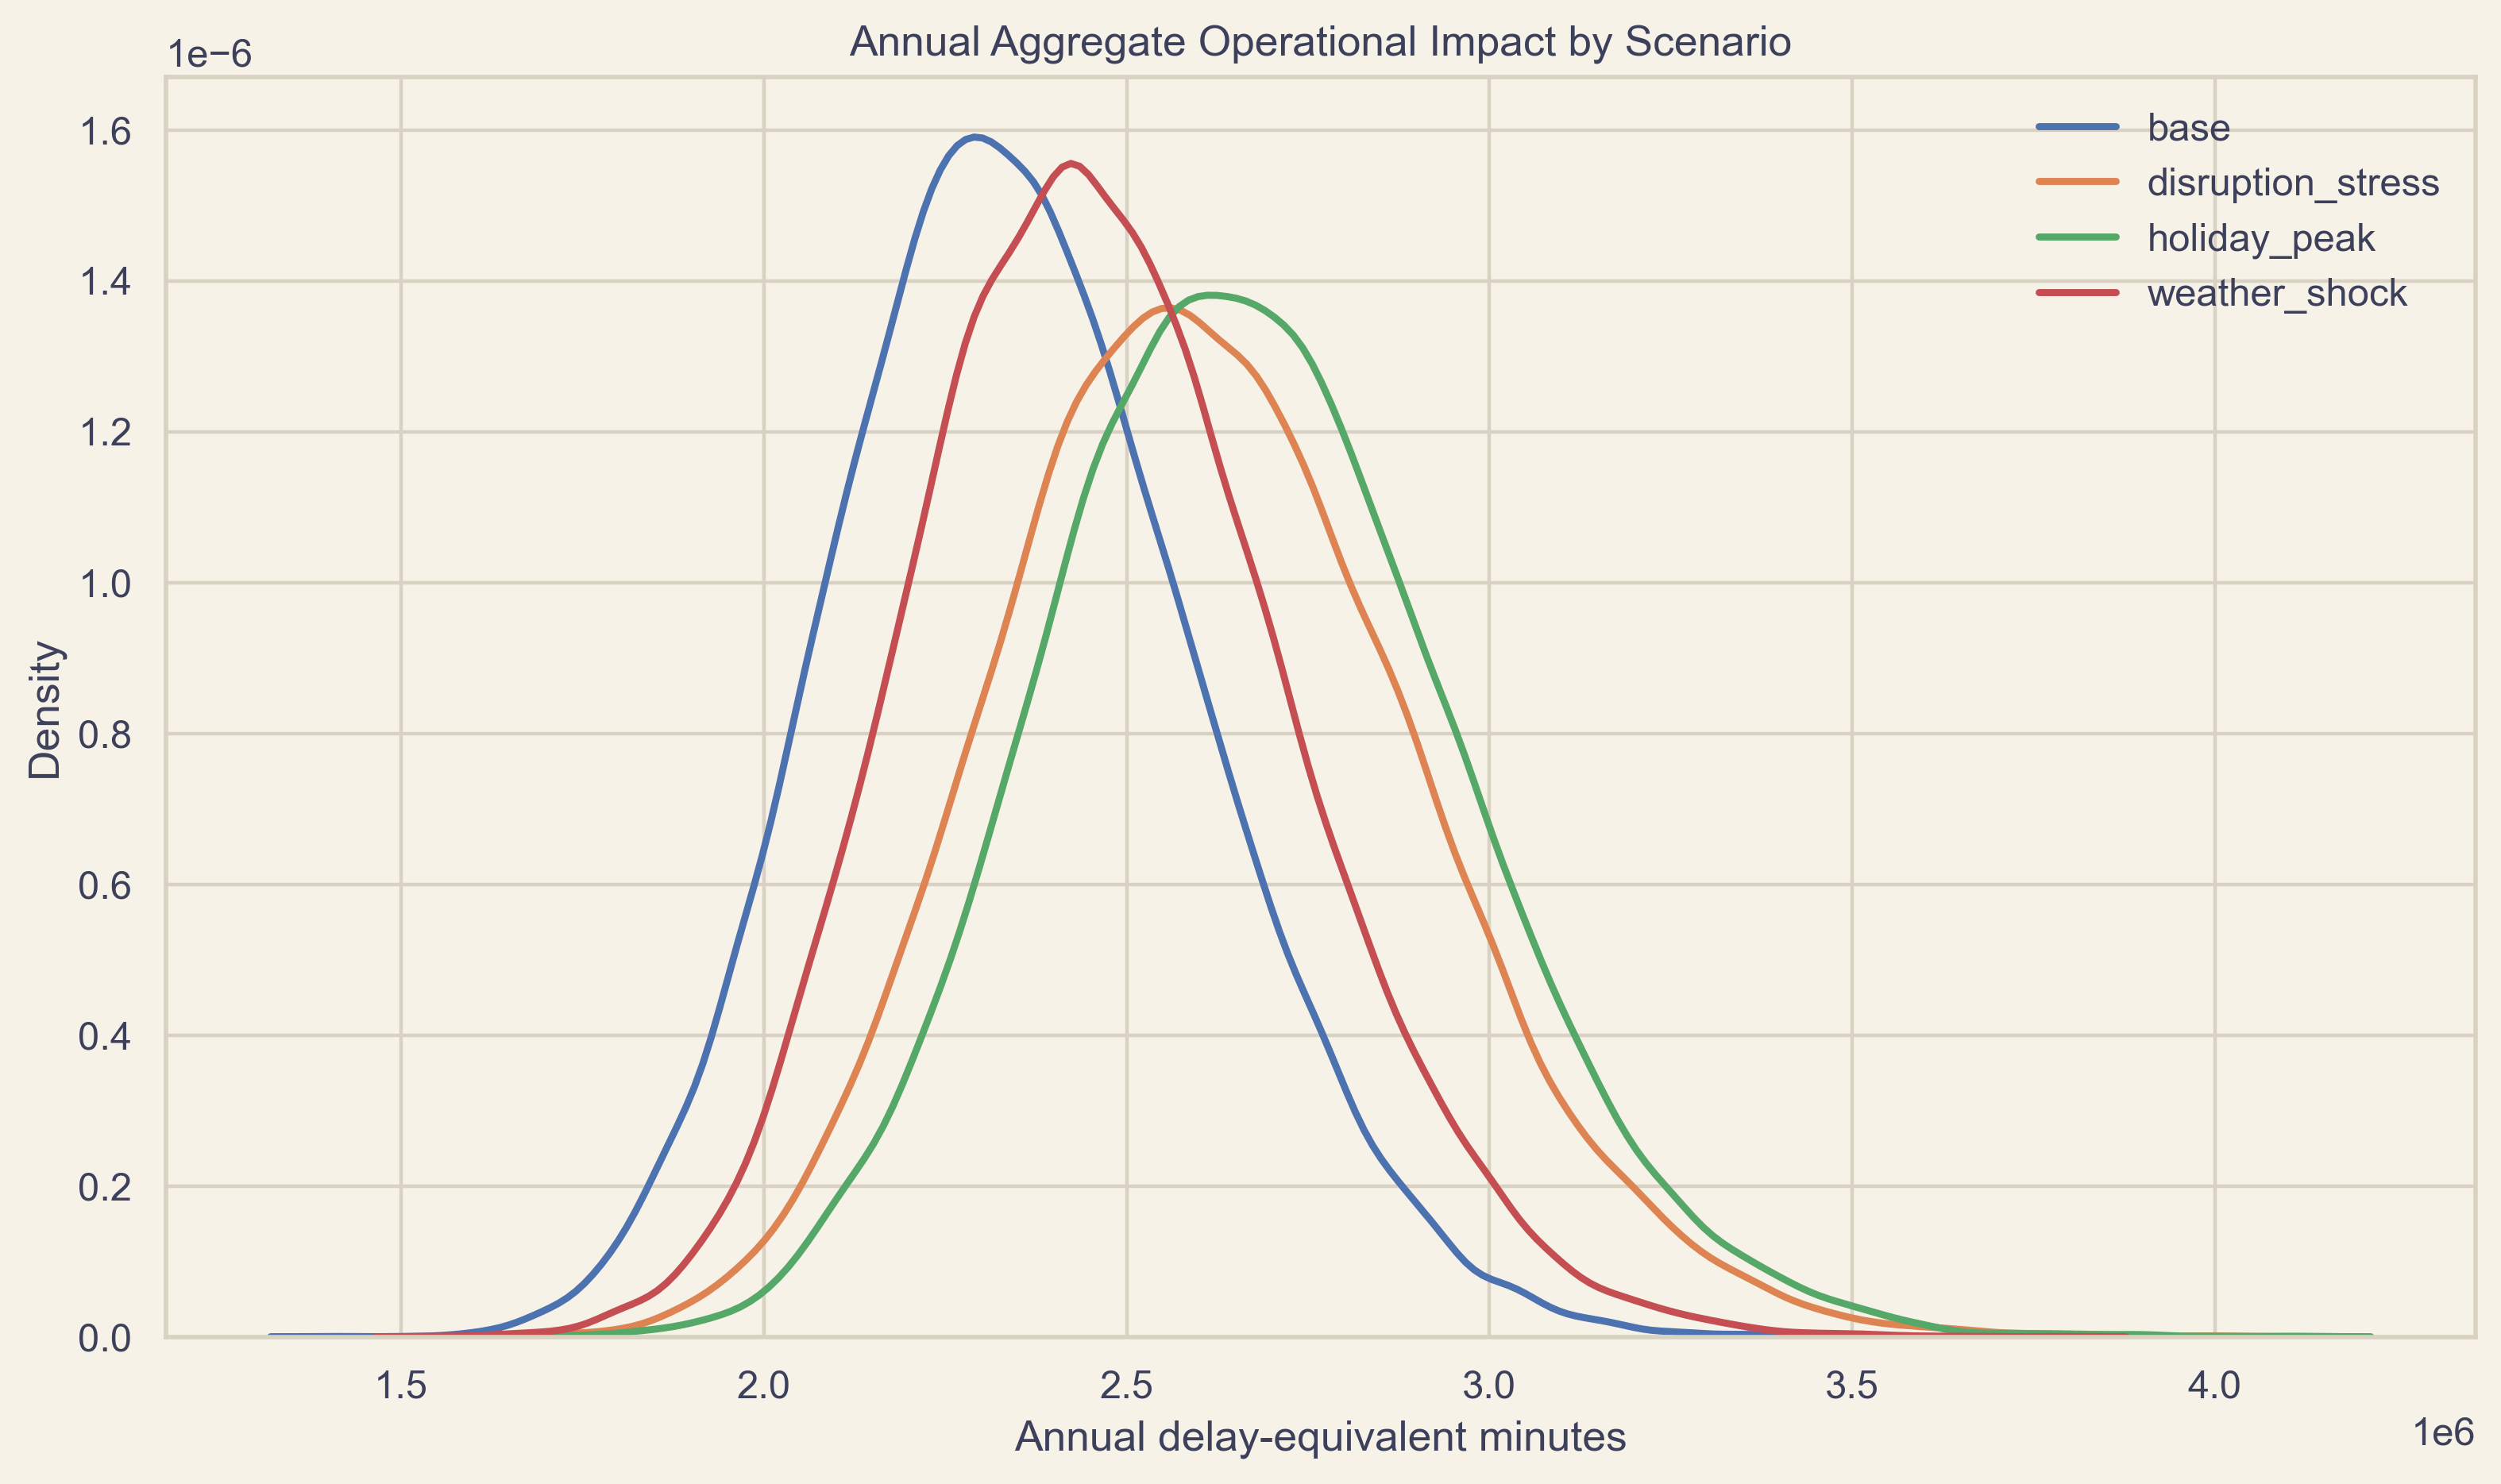
\includegraphics[width=0.90\linewidth]{chart_6_aggregate_risk_scenarios.png}
\caption{Annual aggregate operational-risk distributions by scenario}
\label{fig:agg-risk-en}
\end{figure}

\subsection{EVT Tail Extension}
Because annual operational risk is especially relevant in the tail, the project adds an EVT extension using a peaks-over-threshold approach. Let \(L\) denote simulated annual aggregate impact, and let \(u\) be a high threshold. The exceedance variable is
\[
Y=L-u \mid L>u.
\]
Conditional on exceeding the threshold, the exceedance is modeled by a Generalized Pareto Distribution (GPD):
\[
\mathbb{P}(Y\le y)=1-\left(1+\xi \frac{y}{\beta}\right)^{-1/\xi},
\qquad y>0.
\]
Here, \(\xi\) is the shape parameter and \(\beta\) is the scale parameter.

The threshold is set at the 95th percentile of the simulated annual distribution, and a threshold-sensitivity check is also conducted. EVT is used here as a tail overlay rather than as a replacement for the simulation framework. In other words, EVT is meant to confirm and refine tail interpretation, not to redefine the core model.

\begin{table}[H]
\centering
\caption{EVT tail-fit summary}
\begin{tabular}{lrrrr}
\toprule
Scenario & Shape \(\xi\) & Scale \(\beta\) & Empirical TVaR99 & EVT TVaR99 \\
\midrule
Base & -0.0833 & 134,061 & 3,091,504 & 3,094,013 \\
Disruption stress & -0.0898 & 165,189 & 3,488,504 & 3,492,498 \\
Holiday peak & -0.0873 & 158,518 & 3,519,168 & 3,526,243 \\
Weather shock & -0.0856 & 139,435 & 3,238,526 & 3,236,719 \\
\bottomrule
\end{tabular}
\end{table}

Two points stand out. First, all estimated shape parameters are negative, so the tail is heavy but not explosive. Second, empirical TVaR99 and EVT TVaR99 remain very close in every scenario. That suggests the annual tail produced by the main simulation is already fairly stable, with EVT serving as a useful check rather than a competing story.

\section{Sensitivity Analysis}

\subsection{Why Sensitivity Analysis Is Needed}
The aggregate model and EVT extension provide a tail-risk picture under structured scenarios, but management still needs to know which specific drivers matter most. Sensitivity analysis answers that question by applying targeted shocks to the risk system and measuring how annual expected impact and tail metrics respond.

This step is especially important in operational-risk work because not every modeled component is equally actionable. Some risk blocks matter because they happen often, some because they are severe when they occur, and some because they amplify tail outcomes disproportionately. Sensitivity analysis helps separate those roles.

\subsection{Sensitivity Design}
The project evaluates both single-factor and multi-factor shocks. The single-factor shocks raise one driver at a time, such as internal disruption frequency, system disruption frequency, external disruption frequency, cancellations, or diversions. The combination shocks raise several drivers together to test whether joint stress materially amplifies tail exposure.

For each scenario, the project reports the percentage change relative to the base case:
\[
\%\Delta = \frac{\text{Metric}_{\text{shock}}-\text{Metric}_{\text{base}}}{\text{Metric}_{\text{base}}}\times 100.
\]
This is reported not only for expected annual impact, but also for empirical TVaR99 and EVT TVaR99.

\begin{table}[H]
\centering
\caption{Sensitivity scenarios with the largest EVT TVaR99 increase}
\begin{tabular}{lrrr}
\toprule
Scenario & Expected change & TVaR99 change & EVT TVaR99 change \\
\midrule
Internal +30\% & 15.15\% & 16.21\% & 16.24\% \\
Internal + Cancel +20\% & 14.86\% & 15.22\% & 15.27\% \\
Internal + System +20\% & 13.77\% & 13.71\% & 13.90\% \\
Internal +20\% & 10.20\% & 10.83\% & 10.91\% \\
Cancel +30\% & 6.62\% & 7.42\% & 7.45\% \\
\bottomrule
\end{tabular}
\end{table}

The message is consistent. Internal disruption is the strongest tail-risk driver, and cancellation amplification comes next. Diversion-only shocks matter less by comparison. This is where the modeling starts to speak directly to management. The largest gains are likely to come from aircraft rotation resilience, turnaround buffer design, crew-maintenance coordination, and stronger cancellation recovery capacity.

\begin{figure}[H]
\centering
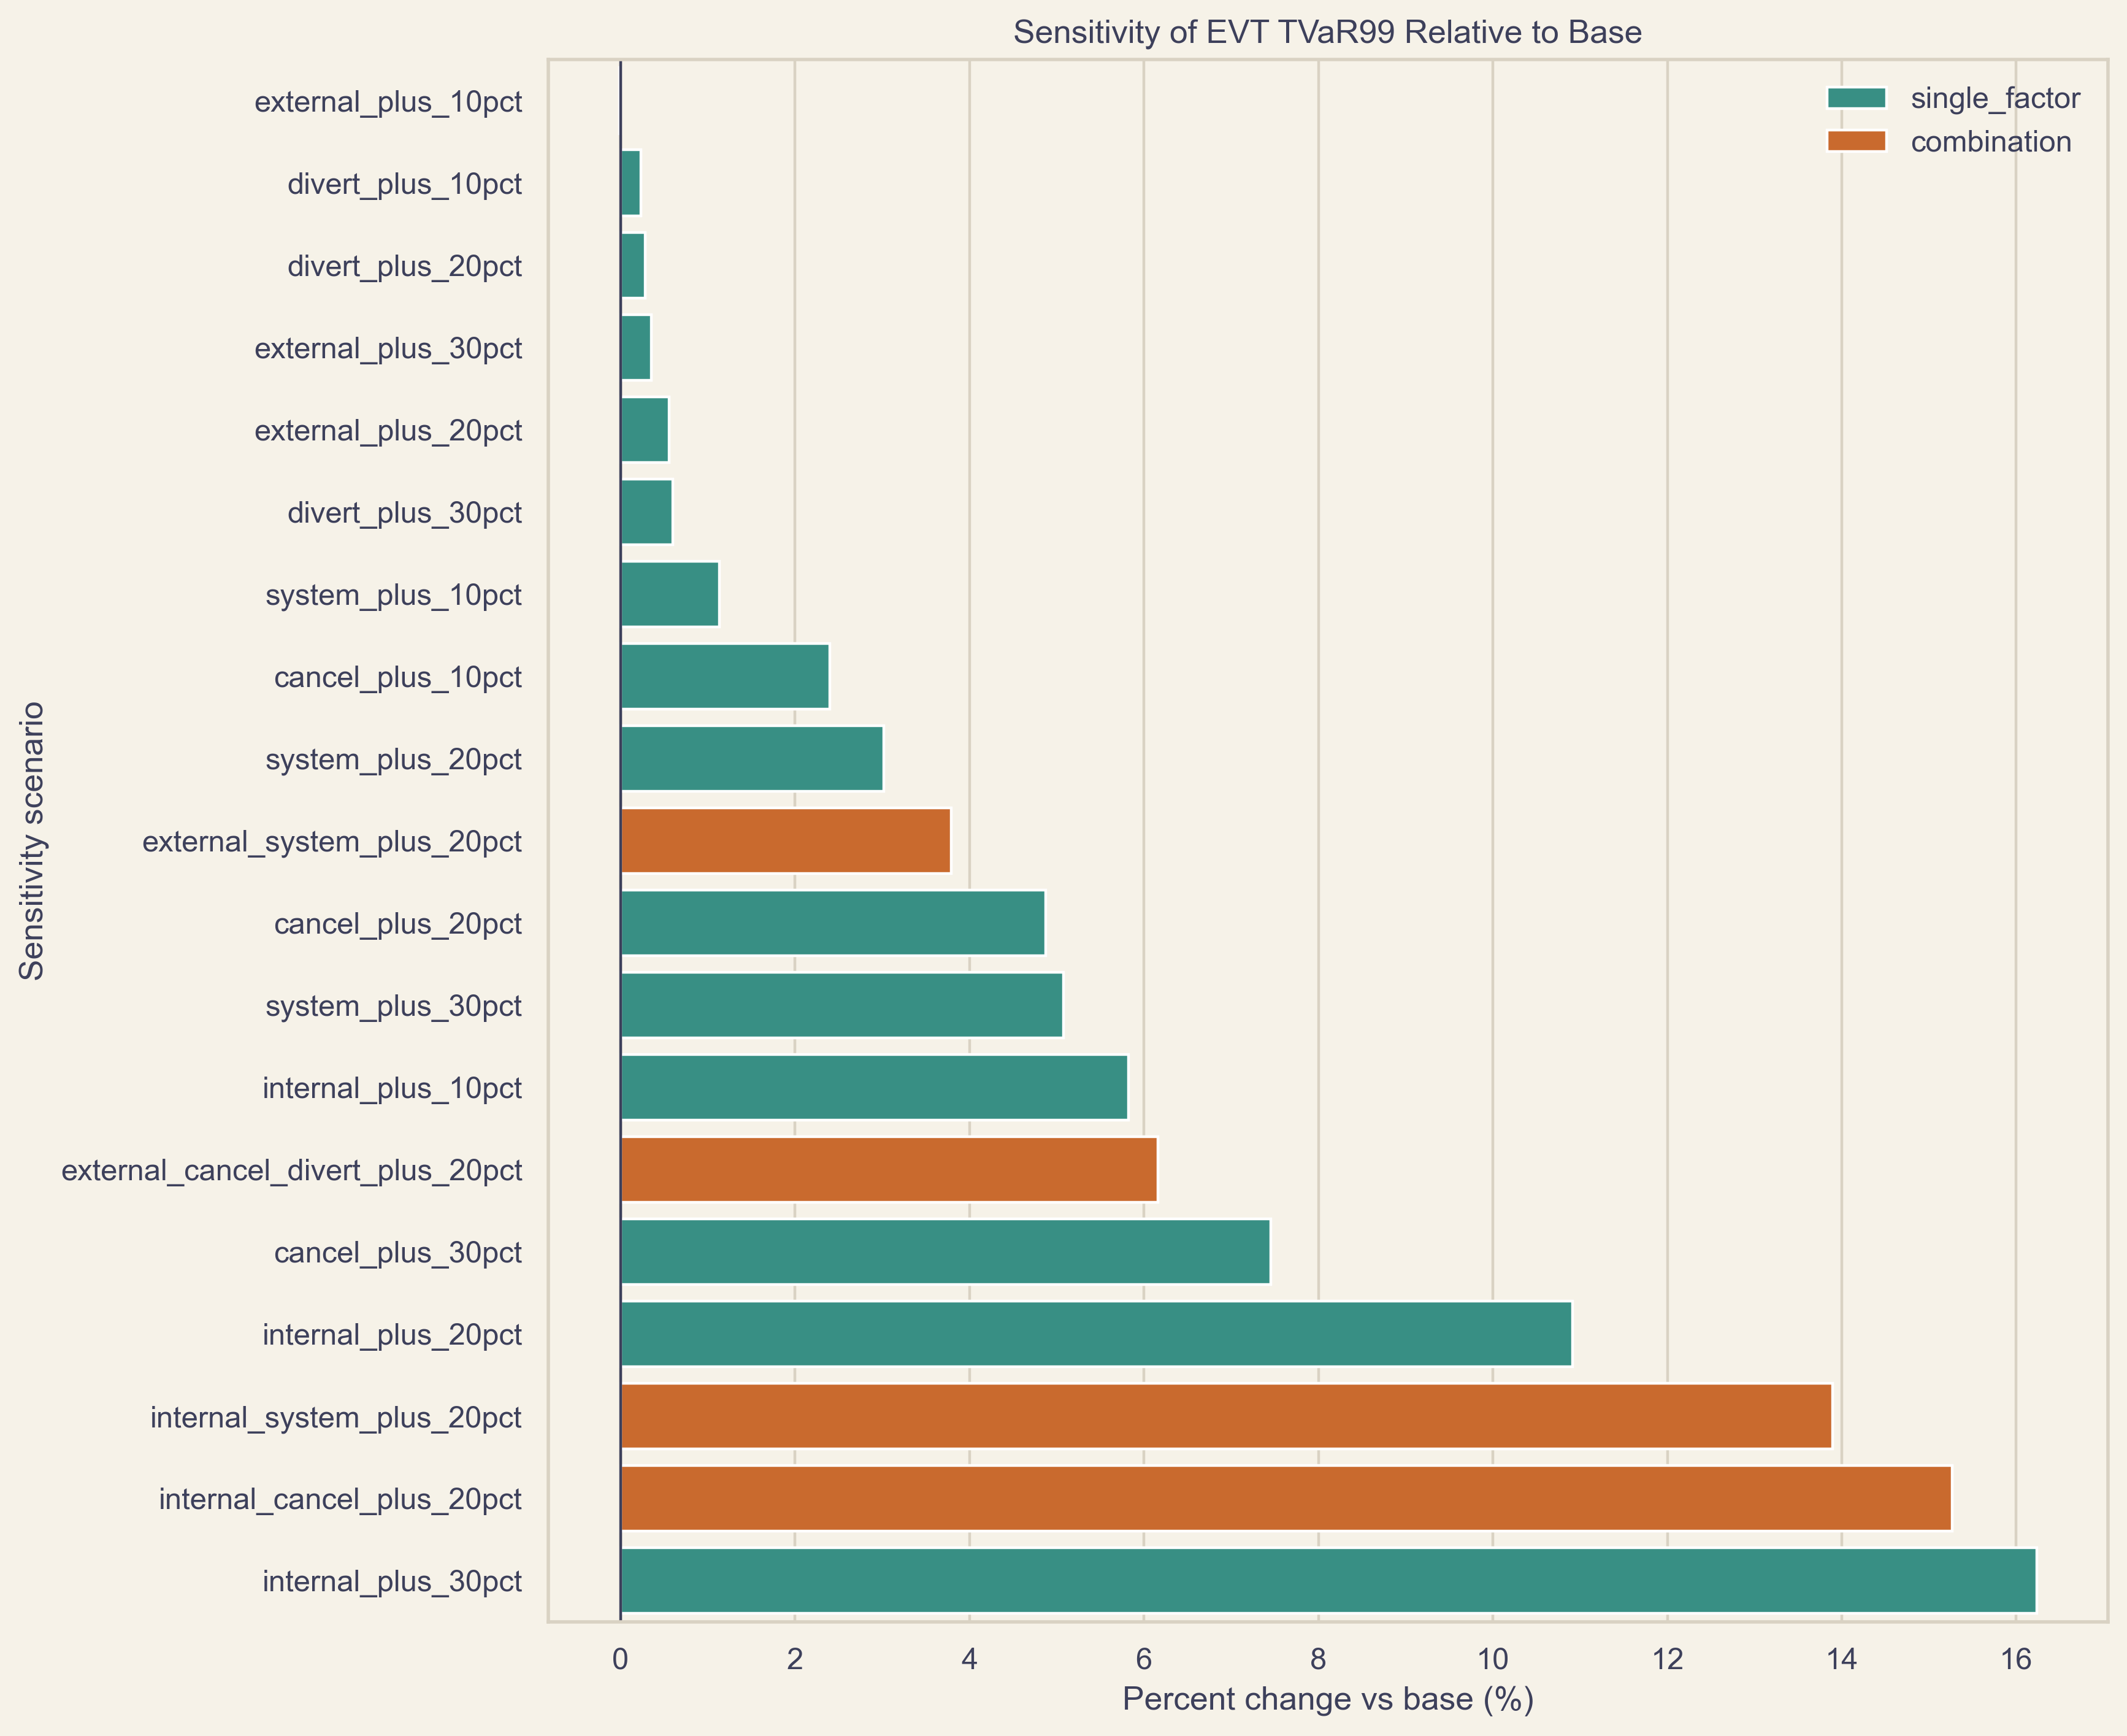
\includegraphics[width=0.90\linewidth]{chart_13_sensitivity_tornado.png}
\caption{Sensitivity of EVT TVaR99 relative to the base scenario}
\label{fig:sensitivity-en}
\end{figure}

\section{Integrated Interpretation and Limitations}
Taken together, the modeling results support a coherent operational-risk story. Disruption counts are clustered rather than homogeneous, which is why the Negative Binomial model dominates the frequency layer. Severity is right-skewed and becomes larger in disrupted months, which supports both flexible severity distributions and a state-based interpretation. Monthly operating conditions display persistence, which makes a simple two-state Markov structure reasonable. At the annual level, aggregate risk is driven more by broad operating stress and peak pressure than by isolated external shocks alone. EVT leaves that picture largely intact, and the sensitivity analysis points to internal disruption and cancellation recovery as the most actionable drivers.

There are, however, several limitations that should be stated openly. First, the loss metric is still a minutes-based operational proxy rather than an observed financial loss measure. Second, the two-state regime structure is intentionally simplified; it captures persistence, but it should not be interpreted as a complete structural model of airport operations. Third, EVT depends on the quality of the underlying annual simulation, so it should be interpreted as a tail extension layered on top of the main model, not as an independent model that supersedes it.

Even with these caveats, the chapter provides a solid quantitative foundation for the rest of the project. It does more than list model outputs. It explains how the model is constructed, why the chosen methods fit the problem, what each layer contributes, and how the empirical results translate into operational-risk terms. That foundation matters for the later discussion, conclusion, and presentation stages.

\end{document}
